%Template pembuatan skripsi dengan ugmskripsi.

\documentclass{jtetiproposalskripsi}
%untuk mengatur agar ukuran kertas menjadi A4 (210mm x 297mm)
\setlength{\paperwidth}{210mm}
\setlength{\paperheight}{297mm}
\usepackage[pass]{geometry}
\usepackage{verbatim,enumerate}
%-----------------------------------------------------------------
%Disini awal masukan untuk data proposal skripsi
%-----------------------------------------------------------------
\titleind{PENGEMBANGAN GATEWAY BERBASIS EMBEDDED DEVICE UNTUK INTEROPERABILITAS JARINGAN SENSOR NIRKABEL DAN PROTOKOL INTERNET}

\titleeng{DEVELOPMENT OF EMBEDDED DEVICE GATEWAY FOR WIRELESS SENSOR NETWORK AND INTERNET PROTOCOL INTEROPERABILITY}

\fullname{GUNTUR DHARMA PUTRA}

\idnum{09/284593/TK/35393}

\approvaldate{13 November 2013}

\degree{Sarjana Teknik Elektro}

\yearsubmit{2013}

\program{Teknik Elektro}

\headprogram{Sarjiya, S.T., M.T., Ph.D.}

\dept{Teknik Elektro dan Teknologi Informasi}

\firstsupervisor{Sarjiya, S.T., M.T., Ph.D.}

\secondsupervisor{Sarjiya, S.T., M.T., Ph.D.}

\firstnip{1983 1020 2008 12 1 002}

\secondnip{1977 0131 2002 12 1 003}
%-----------------------------------------------------------------
%Disini akhir masukan untuk data proposal skripsi
%-----------------------------------------------------------------

\begin{document}

\cover

\approvalpage

%-----------------------------------------------------------------
%Disini akhir masukan untuk muka skripsi
%-----------------------------------------------------------------

%-----------------------------------------------------------------
%Disini awal masukan Intisari
%-----------------------------------------------------------------
\begin{abstractind}
Jaringan sensor nirkabel (Wireless Sensor Network, WSN) adalah jaringan simpul (node) sensor otonom terdistribusi yang digunakan untuk memonitor kondisi fisik atau lingkungan misalnya suhu, suara, getaran, kelembaban, dan lain-lain. Selain itu, tidak menutup kemungkinan untuk menambahkan fungsi tambahan pada setiap simpul misalnya port masukan/keluaran yang dapat digunakan sebagai pengendali aktuator yang terhubung ke piranti elektrik atau elektronis.

Data yang dikumpulkan dari simpul-simpul sensor dalam jaringan tersebut kemudian dibawa ke pengendali utama melalui sebuah gateway untuk diproses lebih lanjut. Data yang terkumpul diharapkan dapat digunakan untuk berbagai keperluan diantaranya untuk home automation dan home surveillance. Letak pengendali utama dapat berada di sekitar tempat WSN atau untuk memudahkan dan meningkatkan fleksibilitas, letak pengatur utama WSN dapat saja berada jauh dari area WSN. Pemilihan jaringan internet sebagai jembatan untuk menghubungkan WSN dengan pengatur utama yang letaknya jauh menjadi sangat tepat karena dewasa ini jaringan internet sudah sangat tersebar. Protokol yang digunakan di internet adalah protokol internet (Internet Protocol, IP). Ada kecenderungan bahwa berbagai komunikasi data akan mengarah menuju konvergensi menggunakan IP. Masalah utama yang dihadapi untuk menghubungkan WSN dengan jaringan IP adalah perbedaan protokol diantara keduanya. Oleh karena itu harus dibangun sebuah gateway yang dapat menjembatani jaringan WSN dengan IP.

Saat ini infrastruktur jaringan data yang sangat populer dan terhubung ke internet adalah jaringan area lokal nirkabel atau dikenal dengan nama WiFi. Salah satu perangkat utama dalam jaringan WiFi adalah access point (AP) yang berfungsi sebagai simpul koordinator. Selain itu, AP juga berfungsi sebagai gateway yang menghubungkan piranti- piranti yang terhubung padanya ke internet. Penelitian ini akan mengembangkan perangkat lunak yang akan ditanamkan (embedded) ke dalam AP sehingga menjadikan AP mempunyai kemampuan sebagai gateway untuk kedua jaringan WiFi dan WSN ke jaringan internet. Di dalam penelitian ini akan digunakan dua buah protokol WSN. 

\bigskip
\textbf{Kata kunci} : bahan magnet, non linear orde dua, optika.
\end{abstractind}
%-----------------------------------------------------------------
%Disini akhir masukan Intisari
%-----------------------------------------------------------------

\tableofcontents
\addcontentsline{toc}{chapter}{DAFTAR ISI}
\selectlanguage{bahasa}\clearpage\pagenumbering{arabic}\setcounter{page}{1}

%-----------------------------------------------------------------
%Disini awal masukan untuk Bab
%-----------------------------------------------------------------
\chapter{LATAR BELAKANG}

\section{Latar Belakang Masalah}
Penggunaan WSN untuk sebuah gedung dan rumah semakin populer karena dapat dimanfaatkan untuk berbagai kepentingan misalnya home automation dan home surveillance. Permasalahan pada WSN adalah jika diinginkan pusat kendali berada pada tempat yang jauh dari jaringan sensornya maka jaringan internet yang memungkinkan untuk menyelesaikan permasalahan ini. Namun demikian, pada umumnya jaringan WSN tidak menggunakan IP sehingga diperlukan gateway yang mampu menghubungkan WSN dengan jaringan internet.

\section{Tujuan Penelitian}
Tujuan penelitian ini adalah untuk mempelajari kemungkinan pengembangan perangkat lunak yang akan ditanamkan ke dalam sebuah AP untuk difungsikan sebagai gateway sehingga mampu digunakan untuk mengintegrasikan jaringan WiFi dan beberapa protokol WSN ke jaringan internet.


\section{Manfaat Penelitian}
Dengan menghubungkan WSN ke jaringan internet maka dimungkinkan untuk mengembangkan aplikasi WSN yang dapat diakses melalui jaringan internet. Terhubungnya WSN ke jaringan internet akan membuka kemungkinan pengembangan layanan-layanan yang lebih beragam terutama layanan yang berbasis IP. Hal ini sejalan dengan perkembangan teknologi komunikasi yang menuju konvergensi penggunaan IP.

Selain itu, pengintegrasian gateway untuk WiFi dan WSN dalam satu piranti juga membuka peluang besar untuk memecahkan persoalan interoperabilitas perangkat keras dan kemudahan sistem.

%-------------------------------------------------------------------------------
\chapter{TINJAUAN PUSTAKA DAN DASAR TEORI}                

\section{Tinjauan Pustaka}
ecara umum, cara untuk menghubungkan WSN dengan jaringan internet dapat dikelompokkan menjadi dua. Cara pertama adalah menggunakan gateway dan cara yang kedua adalah dengan menggunakan simpul sensor yang sudah dilengkapi dengan protokol internet. Cara yang lebih mudah ditempuh adalah dengan cara yang pertama karena pengubahan yang dilakukan relatif tidak terlalu besar. Sedangkan cara yang kedua akan menemui banyak kendala terutama pada WSN yang sudah terpasang karena harus dilakukan penggantian tiap simpul sensor.

Salah satu usaha untuk mengintegrasikan jaringan WSN dengan jaringan WiFi menggunakan gateway misalnya dilakukan pada penelitian [1]. Pada riset tersebut pengintegrasian dilakukan dengan sebuah komputer yang didedikasikan untuk keperluan tertentu. Penggunaan komputer khusus ini adalah hardware-solution yang membutuhkan biaya dan kerumitan sistem.

Riset pada [2] juga menawarkan pengintegrasian dengan jaringan IP. Namun demikian di dalam riset ini diperlukan perubahan yang signifikan jika konfigurasi jaringan sensor nirkabel sudah terpasang. Simpul sensor yang digunakan harus diganti dengan simpul sensor yang mendukung IP. Hal ini jelas akan memakan biaya yang cukup besar dan tidak praktis untuk dilakukan. Terlebih lagi jika jumlah sensor yang terpasang jumlahnya cukup banyak.

Riset pada [3] sudah berhasil mengembangkan sebuah AP menjadi gateway yang dapat digunakan untuk menghubungkan sebuah protokol WSN dengan jaringan IP. Protokol WSN yang digunakan adalah protokol dari IQRF [4]. Penelitian tersebut kemudian dilanjutkan dengan penelitian [5] yang sudah diterapkan dalam sistem domotic.

\section{Landasan Teori}
Jaringan sensor nirkabel (Wireless Sensor Network, WSN) adalah jaringan simpul sensor otonom yang terdistribusi digunakan untuk memonitor kondisi fisik atau lingkungan misalnya suhu, suara, getaran, kelembaban, dan lain-lain. Selain itu, tidak menutup kemungkinan untuk menambahkan fungsi tambahan pada setiap simpul misalnya port masukan/keluaran (I/O port) yang terdapat dalam setiap simpul dihubungkan dengan aktuator sehingga dapat digunakan untuk mengendalikan piranti elektrik atau elektronis.

Secara umum, WSN dapat diilustrasikan seperti Gambar 2. Pada gambar tersebut terlihat adanya beberapa simpul yang diwakili dengan titik berukuran kecil dan satu buah simpul yang diwakili dengan titik berukuran lebih besar. Titik yang berukuran kecil mewakili simpul sensor sedangkan titik yang berukuran besar mewakili gateway yang berfungsi menghubungkan jaringan sensor nirkabel dengan pengendali utama yang dalam gambar tersebut diwakili oleh sebuah komputer. Contoh sebuah simpul dari IQRF [4] ditunjukkan pada Gambar 3.
Gambar 2 Jaringan sensor nirkabel

Pada umumnya, WSN adalah jaringan yang berdiri sendiri. Untuk menghubungkan WSN dengan jaringan yang lain misalnya jaringan internet, maka salah satu cara adalah dengan membangun gateway WSN yang mampu menjembatani perbedaan protokol yang ada pada WSN dan jaringan internet. Cara tersebut adalah cara yang ditempuh dalam penelitian ini karena lebih mudah dilakukan dibandingkan dengan cara yang lain seperti sudah dijelaskan pada Bab Tinjauan Pustaka.

\begin{figure}[ht!]
  \centering
    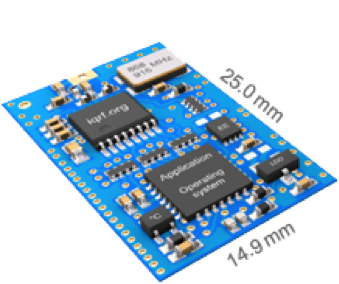
\includegraphics{gambar/iqrf}
    \caption{Contoh sebuah simpul sensor IQRF [4].}
\end{figure}

Sementara itu, jaringan WiFi sebagai jaringan lokal nirkabel yang digunakan untuk komunikasi data dalam suatu area lokal dan sudah tersebar di berbagai tempat. Lokal yang dimaksud disini adalah area yang tidak terlalu luas yaitu dengan radius sekitar 20m atau dalam sebuah gedung. Untuk membangun jaringan lokal menggunakan WiFi, perangkat utama yang digunakan adalah Access Point (AP). AP adalah piranti yang akan menjadi koordinator dalam jaringan lokal jika diinginkan topologi bintang (star) seperti diilustrasikan pada Gambar 4.
Gambar 4 Jaringan bintang menggunakan WiFi.

Gambar 4 memberi ilustrasi sebuah jaringan WiFi yang terdiri dari tiga buah komputer dan satu buah AP yang terhubung ke jaringan internet. Dengan konfigurasi tersebut, semua komputer yang ada di dalam jaringan WiFi dapat berkomunikasi dengan internet dengan aturan yang ditentukan oleh AP.

Jika dilihat lebih dalam lagi, AP ini sebenarnya adalah piranti tertanam (embedded device) yang didalamnya sudah terdapat pusat pengolahan utama, memory, dan penyimpanan (storage). Dengan kenyataan inilah maka AP mempunyai potensi untuk menjagi gateway bagi jaringan WiFi dan WSN ke jaringan internet. Untuk mengembangkan aplikasi yang akan ditanamkan ke dalam AP, maka diperlukan sistem operasi yang sesuai untuk AP.

Sistem operasi yang akan digunakan pada penelitian ini adalah OpenWrt [6] karena sistem operasi ini bersifat open source, tidak berbayar, dan dukungan komunitas yang kuat.

%-------------------------------------------------------------------------------
\chapter{METODOLOGI}

\section{Alat dan Bahan}
Bahan yang digunakan dalam penelitian ini adalah:

\begin{enumerate}[a.]
\begin{singlespace}
\itemsep0em
\item Kit pancar-rima
\item Kit pengembangan program
\item Kit pengunduh program
\item Asesoris kit pancar-rima
\item Kit ekspansi
\item Access Point
\end{singlespace}
\end{enumerate}


\section{Langkah Kerja}
Rancangan arsitektur yang akan digunakan pada penelitian ini diilustrasikan seperti pada Gambar 5. Pada gambar tersebut diilustrasikan sebuah sistem yang terdiri atas dua buah WSN dengan protokol yang berbeda dan satu buah jaringan nirkabel lokal (WiFi). Protokol WSN yang akan digunakan dalam penelitian ini adalah dari IQRF [4] dan ZigBee [7]. Pelaksanaan penelitian ini akan dibagi menjadi tiga paket pekerjaan (Work Package, WP).

\textbf{WP 1: Perancangan Perangkat Lunak}

Pada tahap ini akan dilakukan studi literatur yang dititikberatkan pada sistem operasi (Operating System, OS) untuk piranti tertanam (embedded device). Langkah selanjutnya adalah rerancangan perangkat lunak yang akan ditanamkan pada Access Point (AP). Perangkat lunak yang akan ditanamkan harus bekerja secara efisien karena kemampuan komputasi yang terbatas pada AP.
Gambar 5 Arsitektur WSN dan WiFi dengan sebuah AP

\textbf{WP 2: Implementasi Perangkat Lunak}

Implementasi perangkat lunak dilakukan pada tahap ini. Langkah pertama yang dilakukan adalah memastikan bahwa WSN dapat terhubungan dengan internet sesuai dengan yang direncanakan. Langkah selanjutnya adalah memastikan bahwa jaringan WiFi tidak mengalami gangguan setelah perangkat lunak yang baru tertanam pada AP. Penambahan layanan-layanan yang diperlukan dapat pula dilakukan pada tahap ini.

\textbf{WP 3: Integrasi dan Pengujian Seluruh Sistem}

Jika jaringan WiFi dan dua protokol WSN masing-masing dapat berhubungan dengan internet, maka pada tahap ini akan dilakukan pengujian sistem secara keseluruhan. Pengujian dinaikkan dari skala lab menjadi skala test-bed. Pengujian dalam test-bed dilakukan untuk menjamin bahwa sistem yang dikembangkan bekerja sesuai dengan yang direncanakan.

\section{Jadwal Kegiatan}

%-----------------------------------------------------------------
%Disini akhir masukan Bab
%-----------------------------------------------------------------

%-----------------------------------------------------------------
%Disini awal masukan untuk Daftar Pustaka
%-----------------------------------------------------------------
%%\nocite{Abel2010,Guerbas201350}
%%\bibliography{research-plan}
%%\bibliographystyle{plainnat}
\begin{thebibliography}{99}


	\bibitem[Abraha(1995)]{ab5}
	Abraha, K., 1995, Ph. D. Thesis: \emph{Theory of Surface
	Polaritons and Far Infrared Reflectivity of Antiferromagnets, Rare Earth
	Metals and Ferrimagnets}, University of Essex, England, hal.35 - 79 dan 236 -
	254.  

	\bibitem[Abraha \emph{dkk}(1994)]{ab4}
	Abraha, K., Brow, T. E., Dumelow, T., Parker, T. J. dan Tilley, D. R.,  1994,
	Oblique-incidence Far Infrared Reflectivity Study Of The Uniaxial
	antiferromagnet FeF$_2$, \emph{Physical Review B}, Vol.50, No.10 September
	1994, hal.6808 - 6816. 

	\bibitem[Arkundato(1995)]{ar}
	Arkundato, A.,  1995, Skripsi S1: \emph{Aspek Klasik dan Kuantum Optika Non
	Linear}, Jurusan Fisika FMIPA UGM Yogyakarta Indonesia, hal.2, 9 - 14, 58 - 60
	dan 146.

	\bibitem[Bloembergen dan Pershan(1962)]{blpr}
	Bloembergen, N. dan Pershan, P. S., 1962, Light Waves at The
	Boundary of Nonlinear Media, \emph{Physical Review}, Vol.128, Number 2,
	hal.606 - 622. 

	\bibitem[Bloembergen(1980)]{bl}
	Bloembergen, N., 1980, Conservation laws in nonlinear
	optics, \emph{Journal of Optical Society of America}, Vil.70, No.12 Desember
	1980, hal.1429 - 1436.

	\bibitem[Budker \emph{dkk}(1999)]{bud}
	Budker, D., Orlando, D. J. dan Yaschuk, V., 1999,
	Nonlinear laser spectroscopy and magnet-optics, \emph{American
	Journal Physics}, Vol.67, No.7 July 1999, hal.584 - 592.

	\bibitem[Cotter \emph{dkk}(1999)]{cot}
	Cotter, D., Maning, R. J., Blow, K. J., Ellis, A. D., Kelly, A. E.,
	Nesset, D., Phillips, I. D., Poustie A. J. dan Rogers, D. C., 1999,
	Nonlinear Optics for High-Speed Digital Information Processing,
	\emph{SCIENCE}, Vol.286, 19 November 1999, hal.1523 - 1528.

	\bibitem[Halliday dan Resnick(1986)]{hal}
	Halliday, D. dan Resnick, R., 1986, \emph{Fisika Edisi Ke-3
	Jilid 2}, diterjemahkan oleh Silaban, P. dan Sucipto, E., Penerbit Erlangga,
	hal.537 - 568. 

	\bibitem[Jackson(1999)]{jack}
	Jackson, J. D., 1999, \emph{Classical Electrodynamics}, John
	Wiley and Sons, New York, USA, hal.278 - 282.

	\bibitem[Marjunus(1999)]{mar}
	Marjunus, R., 1999, Skripsi S1: \emph{Analisis Teoretis Optika
	Non Linear Dalam Bahan Megnetik}, Jurusan Fisika FMIPA UGM Yogyakarta
	Indonesia, hal.1 - 76.

	\bibitem[Matlin \emph{dkk}(1997)]{ma}
	Matlin, M. D. dan McGee, D. J., 1997, Photorefractive nonlinear
	optics in the undergraduate physics laboratory, \emph{American Journal
	Physics}, Vol.65, No.7 July 1997, hal.622 - 634.

	\bibitem[Wangsness(1979)]{wangs}
	Wangsness, R. K., 1979, \emph{Electromagnetic Fields}, John
	Wiley and Sons, New York, USA, hal.457 - 475.


\end{thebibliography}
\addcontentsline{toc}{chapter}{DAFTAR PUSTAKA}
%-----------------------------------------------------------------
%Disini akhir masukan Daftar Pustaka
%-----------------------------------------------------------------

\end{document}